\chapter{Technische Anforderungen}
\label{chap:technischeAnforderungen}

Bei den Recherchen der Projektarbeit hat sich die Erkenntnis ergeben, das eine erfolgreiche Verarbeitung von Anfragen die folgenden Komponenten benötigt:
\begin{itemize}
	\item Abbildung der Umwelt mittels Wissensdatenbank
	\item Definieren von Regeln zur Ableitung von Schlüssen mittels Logik
	\item Spracherkennung 
	\item Interne und Externe Schnittstellen zur Kommunikation
\end{itemize}

Die oben genannten Komponenten werden bereits im Ansatz durch die in der Projektarbeit evaluierte Lösung - Apache Stanbol - zur Verfügung gestellt. Allerdings hat sich gezeigt, dass diese grössere Erweiterungen benötigen um die gewünschten Ergebnisse zu liefern.

\section{Architektur}
\label{sec:architektur}
Um verschiedenen Teile zusammen zu nutzen, bietet Apache Stanbol eine frei konfigurierbare Verkettung dieser an. Dies geschieht mittels einer sogenannten Enhancement-Chain. Konkret heisst das, dass eine beliebige Eingabe dieser Kette übergeben werden kann, worauf dann die erste Softwarekomponente der Kette die Eingabe verarbeitet und das Resultat an die nächste Komponente weiterreicht. Diese Vorgang wird durch sämtliche Komponenten der Kette fortgeführt bis schlussendlich das Endresultat an die  anfragende Entität zurückgegeben wird.

Die Arbeit der Bachelorthesis besteht also darin, die Enhancement-Chain und die einzelnen Entitäten zu konfigurieren und zu erweitern.

%enhancementstructure.png/ https://stanbol.apache.org/docs/trunk/components/enhancer/enhancementstructure.png

\section{Abbildung der Umwelt mittels Wissensdatenbank}
\label{sec:architektur_wissensdatenbank}
\subsection{Objekte abbilden}
\label{sec:architektur_wissensdatenbank_Objekte}
Die Abbildung der Umwelt geschieht in Apache Stanbol mittels dem sogenannten Entity Hub.
Dieser stellt Informationen zu Entitäten und Objekten einer spezifischen Wissensdomäne zur Verfügung. Die konkrete Arbeit mit dem Entity Hub besteht also darin Objekte, der für die Arbeit gewählten Domäne, als Entitäten abzubilden.
\subsection{Definieren von Regeln zur Ableitung von Schlüssen mittels Logik}
\label{sec:architektur_regeln}
Um nun aus der Wissensdatenbank Schlüsse ziehen zu können, werden Regeln benötigt. Regeln werden verwendet um mittels Bedingungen auf weitere Eigenschaften schliessen zu können.
Apache Stanbol unterstützt auf Prädikatenlogik basierende Regeln, welche innerhalb der Rule Store Komponente als Rezepte gespeichert werden. Diese sind nichts anderes als eine Zusammenfassung von Regeln, welche eine ähnliche Objektkategorie betreffen.

\section{Spracherkennung}
\label{sec:architektur_spracherkennung}
Um einen Eingabesatz auszuwerten, muss dieser erst als solcher erkannt werden. Konkret müssen also, die einzelnen Wörter als Tokens identifiziert und einer Sprachkategorie zugeorndet werden. Dies geschieht mittels der Spracheerkennungskomponente OpenNLP (open natural language processing). Diese Spracherkennung wird für die Englische Sprache von Stanbol schon weitgehend angeboten. Nach unseren Erkenntinissen ist dies mit der Deutschen Sprache genau so möglich, jedoch nicht gegeben. Dies muss also noch erarbeitet werden. Nach ersten Recherchen wird dazu der Tokenizer sowie der Parser von OpenLNP verwendet.TODO (Link)

\section{Interne und Externe Schnittstellen zur Kommunikation}
 \label{sec:architektur_schnittstellen}
Um die oben genannten Komponenten ansprechen und nutzen zu können, sind Schnittstellen zur Kommunikation unumgänglich.

\subsection{Interne Kommunikation}
\label{sec:architektur_schnittstellen_intern}
Intern nutzt Apache Stanbol, wie bereits beschrieben, die sogenannte Enhancement Chain um von einem gegebenen Input, mittels verschiedenen Komponenten, zu einem Output zu gelangen. Die Enhancement Chain basiert gemäss [TODO:Link] auf einer Graph-Struktur, welche sie zur Kommunikation nutzt.

\subsection{Externe Kommunikation}
\label{sec:architektur_schnittstellen_extern}
Jede Komponente von Apache Stanbol, so z.B. auch die Enhancement Chain sowie deren Einzelkomponenten, verfügt über ein REST-Interface. Dies dient zur Kommunikation gegen aussen. Ein schematischer Ablauf der Kommunikation wird in Abbildung \ref{fig:kommunikationKomponenten} grob dargestellt.

\begin{figure}[H]
	\centering
		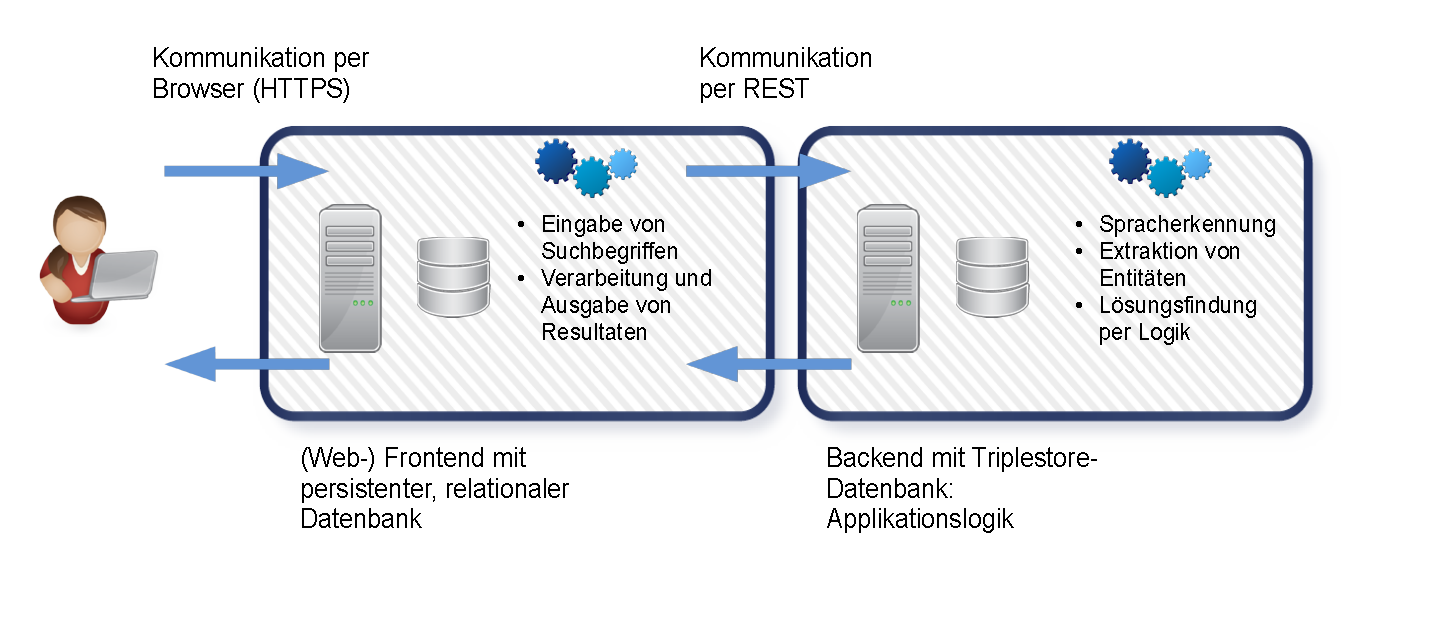
\includegraphics[scale=0.7]{bilder/software_komponenten.png}
	\caption{Kommunikation im Überblick}
	\label{fig:kommunikationKomponenten}
\end{figure}

\chapter{Wissensdomäne}
\label{chap:wissensdomäne}
Wie sich in der Vorarbeit herausgestellt hat, ist es notwendig die Domäne, in welcher Anfragen gestellt werden sollen, sehr detailliert abzubilden. Zudem ist die technische Umsetzung der Suche mittels Apache Stanbol weniger weit ausgearbeitet als ursprünglich angenommen. Um die Komplexität in einem angemessenen Rahmen zu halten, gilt es die Entitäten, also die Modellierung der Umwelt, stark einzuschränken. 
Als Folge dieser Erkenntnisse wird die Wissendomäne, mit welcher gearbeitet wird, eingeschränkt. Bei der gewählten Domäne handelt es sich um die Grundlagen der Programmierung am Beispiel der Programmiersprache Java.

\chapter{Ziel der Thesis}
\label{chap:thesisziel}
Als Endresultat der Thesis soll eine Applikation zur Verfügung stehen, welches es erlaubt eine Frage in deutscher Sprache zur Domäne der Programmierung anhand der Programmiersprache Java zu stellen. Dies kann dank der gegebenen REST-Schnittstelle z.B. direkt per Konsole oder aber per ansprechendem Web-Interface geschehen, welches aber nicht Teil der Thesis ist. Die Applikation soll in der Lage sein mittels der aufgebauten Wissensdatenbank, deren Relationen und schlussendlich Regeln die Frage zu beantworten. Kann eine Frage nicht eindeutig beantwortet werden, sollen zumindest Satzteile (Tokens) extrahiert und der entsprechende Inhalt zu diesen zurückgegeben werden. Eine Antwort ist dabei die Rückgabe einer Entität mit all deren Feldern, welchen dann von dem anfragenden Objekt entsprechend verarbeitet werden kann.
